\documentclass[10pt]{article}
\usepackage{color}
\usepackage{tikz}

% thanks to https://dkumor.com/posts/technical/2018/08/15/causal-tikz/

% Tikz settings optimized for causal graphs.
% Just copy-paste this part
\usetikzlibrary{shapes,decorations,arrows,calc,arrows.meta,fit,positioning}
\tikzset{
  -Latex,auto,node distance =1 cm and 1 cm,semithick,
  state/.style ={ellipse, draw, minimum width = 0.7 cm},
  point/.style = {circle, draw, inner sep=0.04cm,fill,node contents={}},
  bidirected/.style={Latex-Latex,dashed},
  el/.style = {inner sep=2pt, align=left, sloped}
}
\begin{document}

%% \begin{tikzpicture}
%%   % x node set with absolute coordinates
%%   \node[state] (x) at (0,0) {$X$};

%%   % y node set relative to x.
%%   % Locations can be:
%%   % right,left,above,below,
%%   % above left,below right, etc
%%   \node[state] (y) [right =of x] {$Y$};

%%   \node[state] (z) at (0,100) {$Z$};

%%   % Directed edge
%%   \path (x) edge (z);
%%   \path (y) edge (z);

%%   % Bidirected edge
%%   \path[bidirected] (x) edge[bend left=60] (y);
%% \end{tikzpicture}

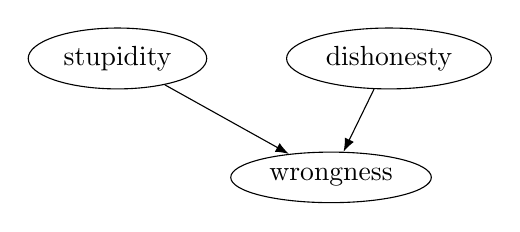
\begin{tikzpicture}

  \node[state] (x) at (0,200) {stupidity};

  \node[state] (y) [right =of x] {dishonesty};

  \node[state] (z) [below right =of x] {wrongness};

  % Directed edge
  \path (x) edge (z);
  \path (y) edge (z);

\end{tikzpicture}



\end{document}
